\apendice{Documentación técnica de programación}

\section{Introducción}
En esta sección, se proporcionará una explicación y una muestra de la estructura organizativa del proyecto, así como el manual del programador y los pasos necesarios para ejecutar el proyecto.

\section{Estructura de directorios}
La estructura del proyecto se divide en diferentes directorios:

\begin{itemize}
    \item \textbf{/Documentación:} carpeta que contiene los documentos de la memoria y anexos del proyecto.
    \item \textbf{/env:} contiene los directorios con ejecutables que determinan que se trata de un entorno virtual.
    \item \textbf{/src:} carpeta que contiene todos los archivos Python relacionados con el funcionamiento del backend de la aplicación.
    \item \textbf{/static:} carpeta que contiene los archivos estáticos relacionados con el frontend, incluyendo el archivo de los estilos aplicados y la carpeta con las imágenes usadas en la aplicación
    \item \textbf{/templates:} carpeta que contiene todos los archivos HTML que forman la parte visual de la aplicación.
    \item \textbf{/translations:} carpeta que contiene los archivos JSON empleados para almacenar las traducciones de los HTMLs, y el archivo que se encarga de cargar las traducciones desde los archivos JSON correspondientes.
    \item \textbf{/uploads:} carpeta oculta que contiene los archivos que subieron los usuarios durante el uso de la aplicación.
    \item \textbf{/videos:} carpeta que contiene los vídeos que muestran el uso de la aplicación.
    \item \textbf{.env:} archivo oculto que contiene las contraseñas necesarias para la conexión a la base de datos.
    \item \textbf{.gitignore:} archivo que contiene el nombre de los archivos que se encuentran ocultos en GitHub.
    \item \textbf{app.py:} archivo principal de Python que contiene todos los métodos GET y POST de la aplicación. 
    \item \textbf{errores.log:} archivo oculto que contiene el registro de los errores que se generan durante la ejecución de la aplicación.
    \item \textbf{LICENSE:} licencia de la aplicación.
    \item \textbf{Procfile:} archivo en el que se determina el archivo principal de la aplicación para el despliegue en Heroku. 
    \item \textbf{README.md:} archivo que contiene la descripción del proyecto junto con los pasos necesarios para su uso.
    \item \textbf{requirements.txt:} archivo que contiene las herramientas junto con sus versiones, para ejecutar el despliegue en Heroku.
   
\end{itemize}

\section{Manual del programador}
En este manual se van a indicar los diferentes procedimientos que debe seguir el programador para la correcta preparación y ejecución del proyecto.

El proyecto ha sido desarrollado inicialmente de forma local en el equipo y posteriormente se ha desplegado en Heroku, por lo que se encuentra disponible en este enlace: \url {https://teachmeplay.herokuapp.com/}. Para la realización de pruebas para cargar correctamente los archivos de los juegos se dispondrá de una máquina virtual como simulación del equipo local.

\subsection{Visual Studio Code}
Visual Studio Code se emplea para el desarrollo de la aplicación web y la creación de todos los archivos y métodos necesarios para el correcto uso y funcionamiento del proyecto.

Para descargar Visual Studio Code, se debe acceder a la página web oficial en \url{https://code.visualstudio.com/download}. Después, se debe seleccionar la versión adecuada para el sistema operativo, en este caso, la versión utilizada es la de Windows.

Una vez completada la descarga, se procede a instalar Visual Studio Code siguiendo los pasos correspondientes.

\subsection{Python}
Como lenguaje de programación se ha utilizado Python. Para descargar Python, se debe acceder a la página web oficial en \url{https://www.python.org/downloads/} y pulsar el botón de descargar la última versión disponible. En este caso, la versión descargada es Python 3.11.3.

Una vez completada la descarga, se procede a instalar Python siguiendo los pasos correspondientes.

\subsection{PostgreSQL}
Para la gestión de la base de datos se ha utilizado PostgreSQL. Para descargar PostgreSQL, se debe acceder a la página web oficial en \url{https://www.postgresql.org/download/} y seleccionar la versión adecuada para el sistema operativo. En este caso, la versión utilizada es la de Windows y la última versión disponible es la versión 15 de 64 bits.

Una vez completada la descarga, se procede a instalar PostgreSQL siguiendo los pasos correspondientes.

Cuando ya se tiene instalado se debe configurar para poder acceder a la base de datos de Heroku. 

Para ello, se debe crear un nuevo servidor.
\newpage
    \begin{figure}[htbp]
    \centering
    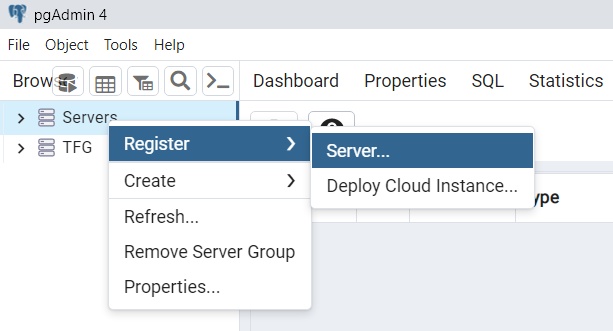
\includegraphics[width=0.7\textwidth]{server}
    \caption{Crear nuevo servidor.}
    \label{fig:server}
    \end{figure}

Este se configura con los datos que obtenemos del Add-on de Heroku. Se debe rellenar el nombre del servidor en la pestaña ``General``.
    \begin{figure}[htbp]
    \centering
    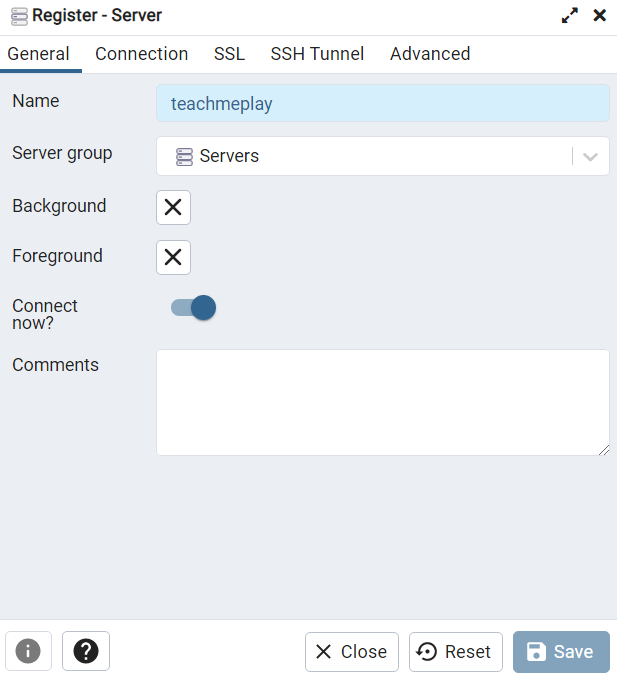
\includegraphics[width=0.3\textwidth]{server1}
    \caption{Crear nuevo servidor: general.}
    \label{fig:server1}
    \end{figure}
    
Se debe rellenar el nombre del host, el puerto, el nombre de usuario, base de datos y la contraseña en la pestaña ``Connection``.
\newpage
    \begin{figure}[htbp]
    \centering
    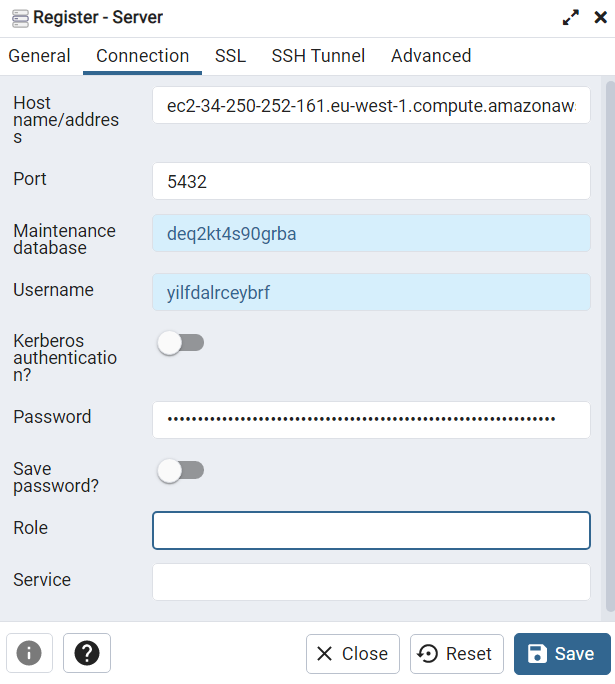
\includegraphics[width=0.3\textwidth]{server2}
    \caption{Crear nuevo servidor: connection.}
    \label{fig:server2}
    \end{figure}
    
Y, por último, se debe rellenado el campo de DB restriction en la pestaña ``Advanced``.
    \begin{figure}[htbp]
    \centering
    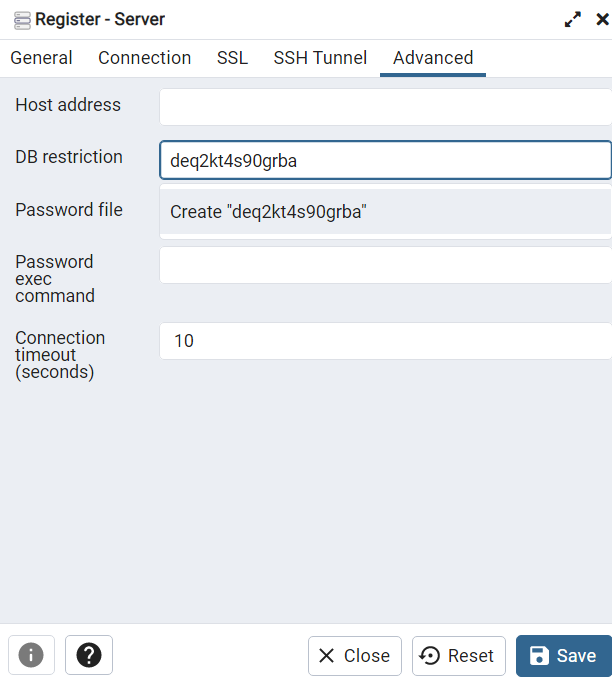
\includegraphics[width=0.3\textwidth]{server3}
    \caption{Crear nuevo servidor: advanced.}
    \label{fig:server3}
    \end{figure}

\subsection{Virtual Box}
El proyecto está disponible en una máquina virtual para poder realizar pruebas en local. De esta forma se permite cargar los distintos archivos de los juegos que se admiten en la aplicación, que debido a las limitaciones de Heroku, no se permite comprobar su funcionamiento en la aplicación desplegada.

Para ello, se empleará VirtualBox, que ha sido utilizado en diversas asignaturas del grado. Esta herramienta ofrece una interfaz de usuario sencilla y un buen rendimiento.

Para su instalación se debe acceder a la página oficial disponible en \url{https://www.virtualbox.org/}, en la sección de descargas,  seleccionar la versión y paquete deseado siguiendo los pasos que se indican.

Como sistema operativo se ha usado Windows 10 Pro obtenido mediante la compra de una licencia OEM. La descarga de la ISO se realiza a través de la página oficial \url{https://www.microsoft.com/es-es/software-download/windows10} seleccionando la última versión disponible.

Una vez se tiene todo instalado se debe crear una máquina dentro del VirtualBox a través del botón de ``Nueva``, asignado el nombre de la máquina virtual y el sistema operativo que se va a instalar.
    \begin{figure}[htbp]
    \centering
    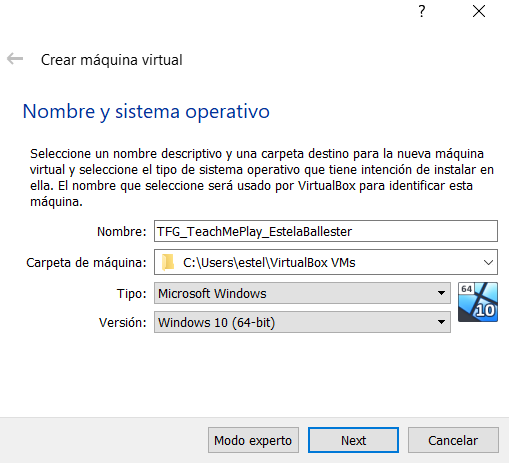
\includegraphics[width=0.6\textwidth]{vb}
    \caption{Creación de máquina virtual.}
    \label{fig:vb}
    \end{figure}
    
Posteriormente se deben seguir los pasos seleccionando la RAM que se desea y la creación de un disco duro VDI. Para instalar el sistema operativo de Windows 10 en la máquina creada, se debe hacer a través de la configuración añadiendo una unidad óptica y seleccionando el archivo ISO que se obtuvo anteriormente.

Por último, cuando se inicie la máquina virtual creada aparecerá la instalación de Windows, por lo que será necesario introducir la clave de la licencia comprada.

Cuando la máquina virtual ya está lista para su uso, se procede a la instalación de Python, Visual Studio Code y PostgreSQL, siguiendo los pasos descritos anteriormente. Después, se importan todos los archivos necesarios en la máquina y se configura la base de datos.

Finalmente, se exporta la máquina virtual mediante la opción de ``Exportar servicio virtualizado``.

\section{Compilación, instalación y ejecución del proyecto}
Para la ejecución del proyecto, se puede realizar de dos formas.
El proyecto puede ejecutarse en local desde la máquina virtual que se proporciona, o mediante el enlace de la página web en el que se encuentra desplegado en Heroku.

\subsection{Ejecución en local}
Para la ejecución en local se proporciona una máquina virtual de VirtualBox con sistema operativo Windows 10 y con todas la herramientas necesarias instaladas.

El objetivo de la máquina virtual es que se pueda ejecutar de forma rápida en local para probar todas las funcionalidades de la aplicación, ya que debido a las restricciones de Heroku no se permite ni cargar ni descargar los archivos de los juegos en la aplicación desplegada.

Para acceder a la sesión de la máquina virtual se debe introducir el PIN: ``0806``.
Una vez iniciada la sesión para ejecutar la aplicación se debe abrir Visual Studio Code e ingresar en el terminal los comandos:
\begin{itemize}
    \item env\textbackslash Scripts\textbackslash activate
    \item flask run
\end{itemize}

También, en el escritorio de la máquina se dispone de un archivo ``ejecutable.bat``, para que al acceder a éste, se ejecuten los comandos necesarios para activar tanto el entorno virtual como para ejecutar el proyecto.

El acceso a la aplicación web está disponible a través del siguiente enlace \url{http://127.0.0.1:5000/}

\subsection{Despliegue en Heroku}
Para desplegar la aplicación en Heroku es necesario obtener el paquete de desarrollo para estudiantes de GitHub para obtener beneficios por ser estudiante, lo cual permite obtener unos créditos para usar dentro de Heroku ya que se van a usar funcionalidades de pago.

Para desplegar el proyecto en Heroku, lo primero que se debe hacer es
registrarse en su página web en el siguiente enlace: \url{https://www.heroku.com/home}

Después de haberse registrado e iniciado sesión, para crear una aplicación se debe pulsar el botón New, donde habrá que establecer un nombre para la aplicación y elegir una región.
    \begin{figure}[htbp]
    \centering
    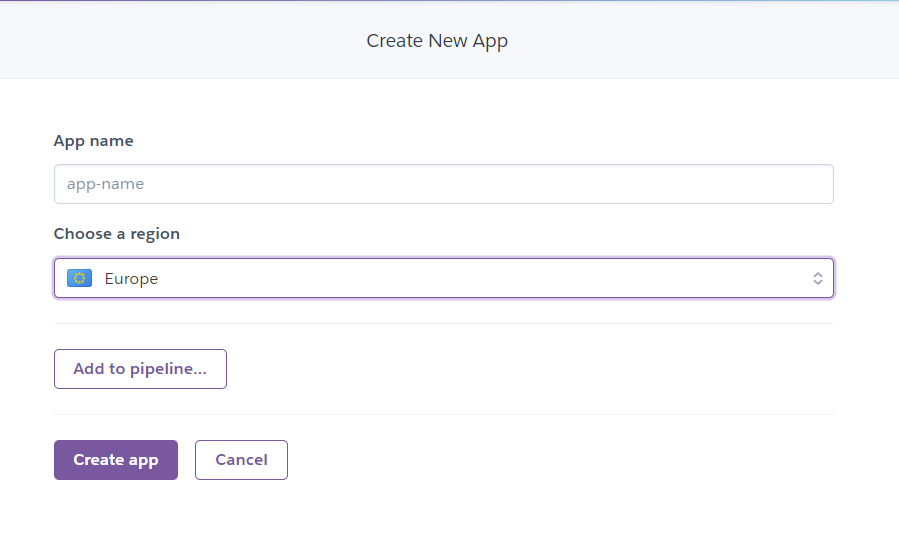
\includegraphics[width=0.7\textwidth]{new-app}
    \caption{Crear nueva aplicación en Heroku.}
    \label{fig:new-app}
    \end{figure}

Una vez creada la nueva aplicación, en la pestaña ``Deploy``, se muestran las opciones y los pasos a seguir para ejecutar el proyecto. Para ello, se debe elegir el método de despliegue en nuestro caso será con GitHub.
\newpage
    \begin{figure}[htbp]
    \centering
    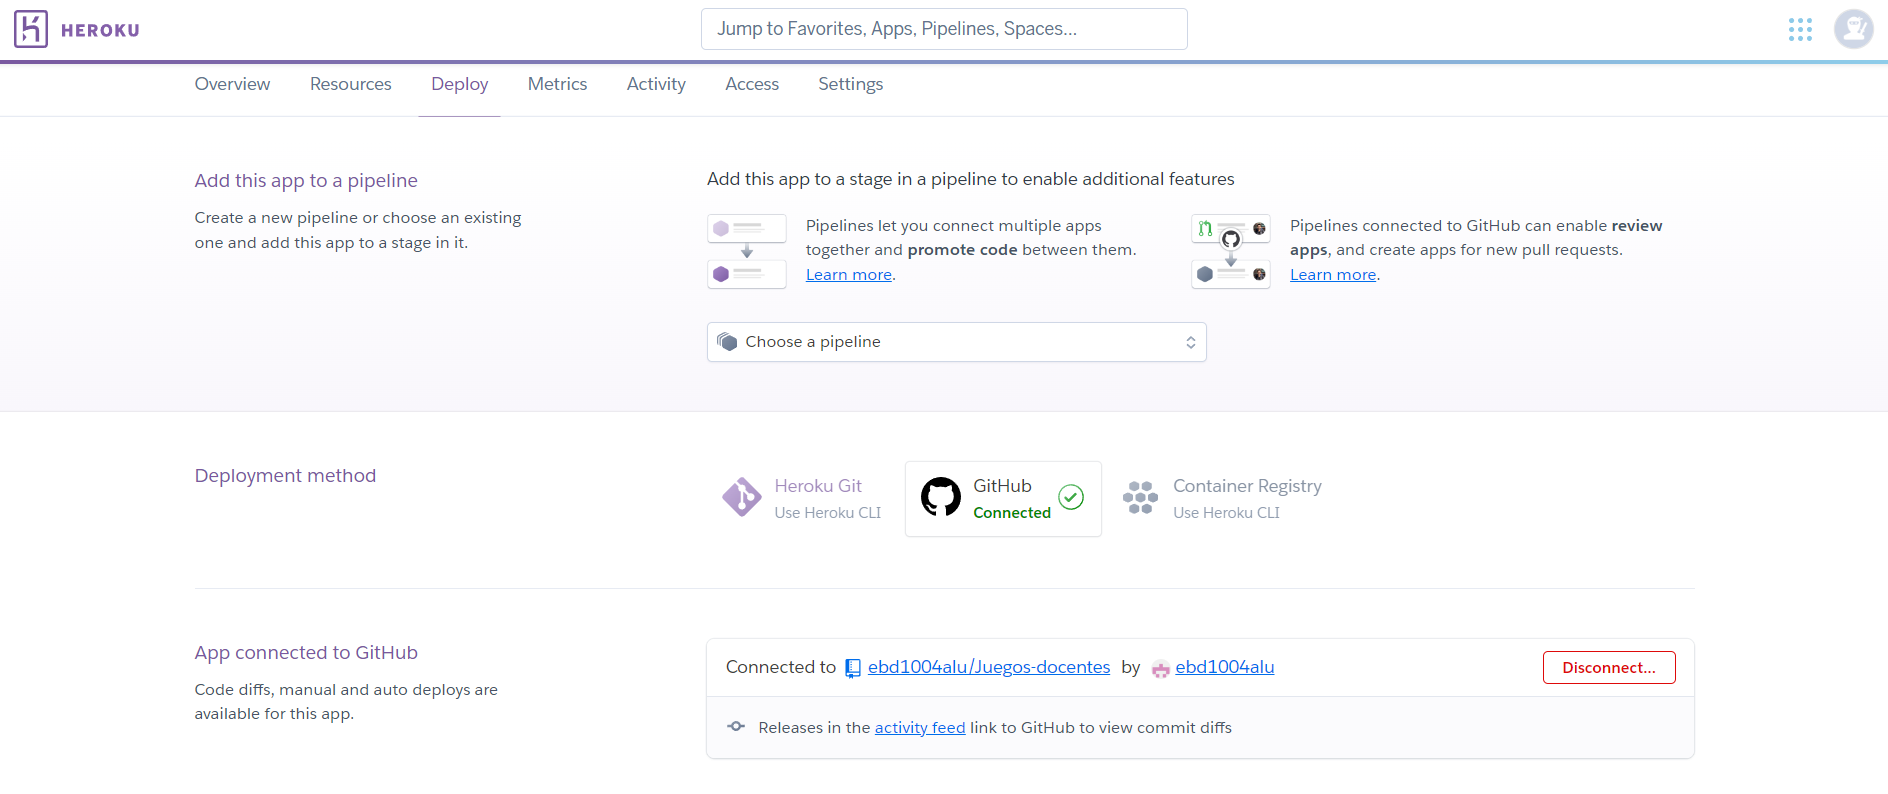
\includegraphics[width=0.8\textwidth]{deploy}
    \caption{Despliegue aplicación en Heroku.}
    \label{fig:deploy}
    \end{figure}


Para el acceso a la base de datos se debe incluir en Heroku un add-ond de Heroku-PostreSQL y así poder desplegar la base de datos en la nube. 
\imagen{add-on}{Add-on Heroku Postgres}

Tras obtener las credenciales de Heroku-PostgreSQL se deberán configurar las variables de entorno de Heroku.
    \begin{figure}[htbp]
    \centering
    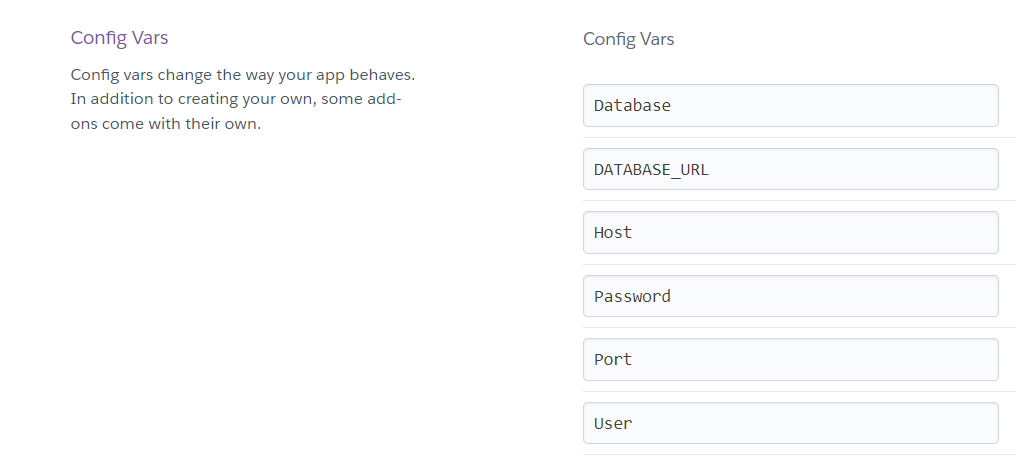
\includegraphics[width=0.8\textwidth]{vars}
    \caption{Configuración variables de entorno.}
    \label{fig:vars}
    \end{figure}

Una vez se ha configurado todo, ya se puede desplegar el
proyecto pulsando sobre el botón de ``Deploy Branch``.
    \begin{figure}[htbp]
    \centering
    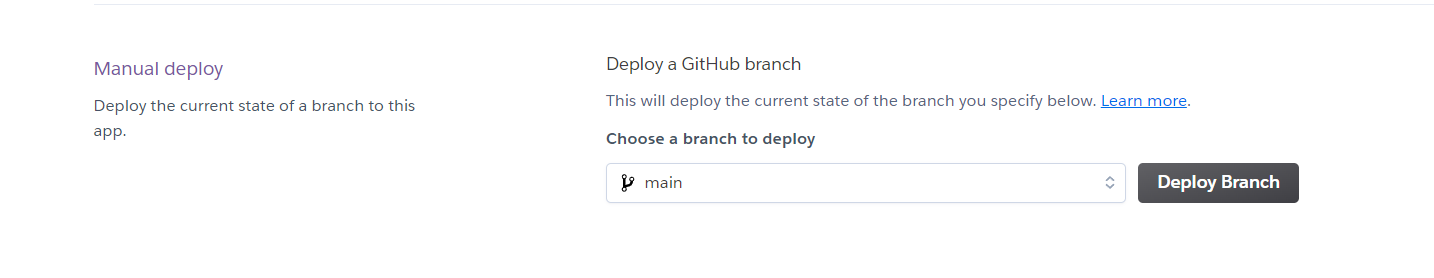
\includegraphics[width=0.9\textwidth]{deploy-branch}
    \caption{Despliegue aplicación en Heroku.}
    \label{fig:deploy-branch}
    \end{figure}
    
\section{Pruebas del sistema}

Para comprobar que la aplicación funciona correctamente, se han realizado una serie de pruebas:

\begin{enumerate}
    \item Se introdujo incorrectamente los credenciales al iniciar sesión para verificar que no permite iniciar sesión y muestra un mensaje de error.
    \item Se introdujo incorrectamente los credenciales al iniciar sesión tres veces para comprobar que no permite iniciar sesión y bloquea al usuario durante 1 minuto, mostrando un mensaje de error.
    \item Se introdujo un nombre de usuario que ya existe al registrarse para comprobar que no permite el registro y muestra un mensaje de error.
    \item Se introdujo una contraseña que no cumple con los requisitos al registrarse para comprobar que no permite el registro y muestra un mensaje de error.
    \item Se introdujo una contraseña distinta a la de confirmación al registrarse para comprobar que no permite el registro y muestra un mensaje de error.
    \item No se introdujo uno de los campos requeridos al registrarse para comprobar que no permite el registro y muestra un mensaje de error.
    \item Se realizó una búsqueda que no existe para comprobar que no muestra resultados y muestra un mensaje de error.
    \item Se probó que los resultados buscados se encontraban correctamente tanto por la barra de búsqueda como por los filtros.
    \item Se probó que se visualizaba correctamente la información de cada juego.
    \item Se probó que el usuario podía valorar correctamente los juegos una vez.
    \item Se probó que el usuario podía solicitar el rol de profesor una vez y que el administrador podía aprobarlo.
    \item Se probó que el profesor pudiera añadir un juego, modificarlo y añadir archivos al juego.
    \item Se probó a cargar archivos que excedieran el límite de tamaño, tuviesen un nombre demasiado largo y un tipo no admitido.
    \item Se probó que el administrador pudiera borrar juegos y usuarios.
\end{enumerate}


